\subsection{MetaDE}

MetaDE package implements 12 major meta-analysis methods for differential expression analysis falling into 3 main categories: combining p-values, combining effect sizes and others (e.g. combining ranks, etc.). Depending on the types of outcome, the package can perform two class comparison, multi-class comparison, association with continuous or survival outcome. The package allows the input of either microarray (continuous intensity) and/or RNA-seq data (count) for individual study analysis. 
The R package for MetaDE module can be found \url{https://github.com/metaOmics/MetaDE}.
After obtaining DE genes from meta-analysis, 
users can further perform pathway enrichment analysis based on the declared DE genes.
In the two subsections below we will go over how to perform (1) meta-analysis and (2) pathway enrichment analysis based on (1).


\subsection{Meta-analysis for differential expression}

\begin{figure}[H]
\begin{center}
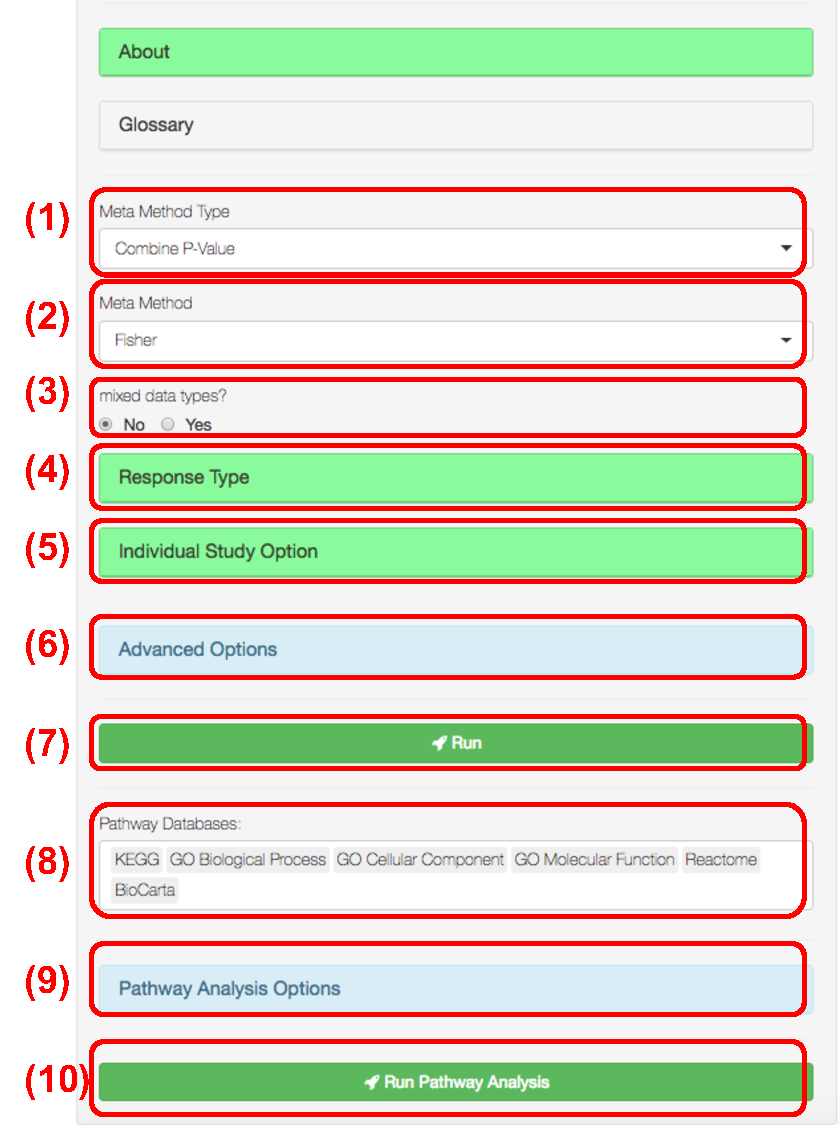
\includegraphics[scale=0.5]{./figure/metaDE/metaDEoption.pdf}
\caption{``MetaDE" options}
\label{fig:MetaDEoption}
\end{center}
\end{figure}

\subsubsection{Procedure}
In Figure~\ref{fig:MetaDEoption},
{\color{red} (1) - (6)} are the steps to tuning parameters and run meta-analysis.
A detailed list of all options available for the package can be found at the end of this subsection. 

\begin{steps}
\item \textbf{Choose the type of meta-analysis methods:}
There are three types of meta-analysis to choose:
combining p-values, combining effect size and others.

\item \textbf{Choose a meta-analysis method:}
\begin{itemize}
\item For ``combining p-values" category,
users can choose from ``Fisher", ``AW-Fisher", ``maxP", ``minP", ``roP" and ``Stouffer",
where some of them have the one-sided corrected versions.

\item For ``combining effect size" category,
users can choose from ``FEM" and ``REM",
where ``REM" has choice of six analytical algorithms for implementation.

\item For ``others",
there are three rank-based method (PR, SR and rankProd) and minMCC for multi-class meta-analysis.
To choose from the overwhelmingly many meta-analysis methods,
we follow \cite{chang2013meta} and mark * for top performing methods AW-Fisher, REM (HO option) and roP as recommendation for users.
\end{itemize}

\item \textbf{Mixed data type:}
If this option is selected,
MetaDE will allow partial studies with count data from RNA-seq and remaining studies with continuous intensities from microarray.

\item \textbf{Choose the response type:}
Under the drop-down menu,
users can specify types of outcome (response) variable to be two-class, continuous, multi-class or survival.
By choosing ``two class comparison",
users can specify the group label name for the Label Attribute (from the column names of your clinical data).
Then for group label (a factor of at least two levels),
specify the name for the ``Control Label" and ``Experimental Label", respectively.
For the other types, only group label name is needed.

\item \textbf{Choose Study Design for individual study:}
\begin{itemize}
\item Individual data type can be either discrete (count) or continuous.
\item Under drop-down menu ``Setting Individual Study method", user can specify  individual study method according to individual data type.
For continuous data (e.g. microarray), available options include LIMMA (default method) and SAM.
For discrete data (e.g. RNA-seq count), available options include edgeR, DESeq2 and voom.
\item The users can also specify whether each study is paired design or not.
\end{itemize}

\item \textbf{Advanced Options}
\begin{itemize}
\item Use complete options: other uncommonly used options will become available. Again, this is not suggested if you are not familiar with the method.
\item Parametric: if No is selected, permutation will be performed instead of parametric closed form solution.
\item Covariate: indicate if any covariate will be adjusted.
\item Alternative Hypothesis: two-sided or one-sided.
\end{itemize}


\end{steps}



\textbf{Step 1. Meta differential analysis:} This step includes the core strategies of the ``MetaDE" package. Users first need to specify (1) ``Meta Method Type" and (2) ``Meta Method" correspondingly. There are three types to select from: combining p-value, combining effect size and others. ``Fisher" and ``AW-Fisher" meta methods are available for p-value combination, ``Fixed Effect Model (FEM)" and ``Random Effect Model (REM)" for effect size combination, and the other methods in the ``Others" type. More meta-analysis methods are available if ``complete option" is chosen from (5) ``Advanced Options" section. Next, we need to specify the outcome of interest in (3) ``Response Type". For example, for differential expression analysis, two-class comparison is usually chosen. For two-class comparison, users need to specify the class label, and the level corresponding to the experimental and the control groups. Other outcome types such as continuous or survival data can also be chosen. In (4) ``Individual study option", users can specify whether each of the study is a paired design, and for p-value combination method, one can select the differential analysis method to obtain p-values in each individual study (e.g. generally suggest LIMMA for microarray and edgeR for RNA-seq). ``Advanced Options" is optional and users are suggested not to modify the option setting in this section. Once all the above options are specified, users can click on (6) ``Run" to implement the first step. \\~\\

\textbf{Step 2. Pathway analysis:} This step consists of a downstream pathway analysis for the meta differential analysis results from the first step. Users can select from 25 available pathway databases (7) to perform the pathway enrichment analysis. There are three main options for pathway analysis under (8) ``Pathway Analysis Option": the enrichment method including the Fisher's exact test and KS test, the minimum as well as the maximum pathway size. If ``Fisher's exact test" is chosen for the enrichment method, users need to further specify the criteria for selection of DE genes: either by p-value cutoff or by number of top ranked genes. Once these options are set, users can click on (9) ``Run Pathway Analysis" to implement the first step. \\~\\


\textbf{Complete List of Options:} 

\begin{enumerate}
  \item Meta Method Type: Combining p-value, Combining effect size, Others.
  \item Meta Method: Fisher, AW-Fisher, FEM, REM, Sum of Rank, Produce of Rank, multi-class correlation, Rank product. 
  \item Response Type:
   \begin{itemize}
     \item Two class comparison, Multi-class comparison, Continuous outcome, Survival outcome.
     \item Label Attribute: select the label name of the outcome.
     \item Control Label \& Experimental Label: specify the case/control label for two-class comparison.
    \end{itemize}
   \item Individual Study Option:
     \begin{itemize}
     \item Setting individual study method
     \item Setting individual study paired option
    \end{itemize} 
   \item Advanced Option (**Optional):
     \begin{itemize}
      \item Use complete options
      \item Parametric
      \item Covariate
      \item Alternative hypothesis
    \end{itemize} 
    \item Run
    \item Pathway Databases
    \item Pathway Analysis Option:
         \begin{itemize}
      \item Pathway enrichment method
      \item Pathway min gene size
      \item Pathway max gene size
    \end{itemize} 
    \item Run Pathway Analysis
\end{enumerate}


\subsubsection{Results}

\begin{figure}[H]
\begin{center}
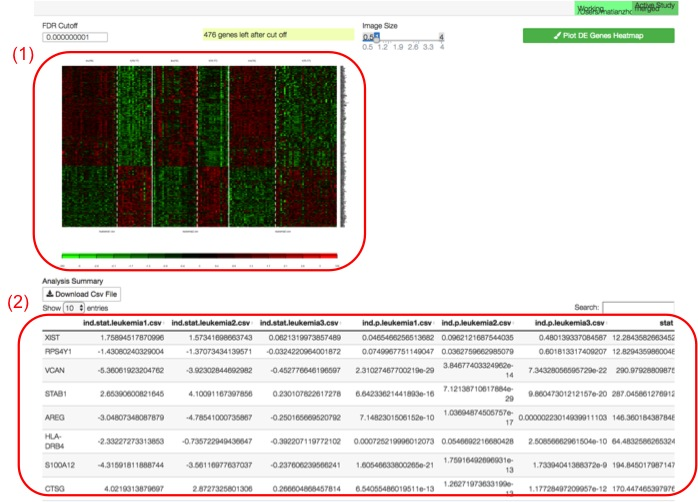
\includegraphics[scale=0.45]{./figure/metaDE/metaDEresult1.jpg}
\caption{``MetaDE" Results (1)}
\label{fig:MetaDEresult1}
\end{center}
\end{figure}

Two main outputs from the first ``meta differential analysis" step in the procedure are shown in Figure \ref{fig:MetaDEresult1}. The first is (2) a summary of meta analysis results, including information of individual test statistics, individual study p-value, meta-analysis p-value, FDR, etc. The second output is (1) a heatmap of DE genes drawn after specifying the FDR cutoff for selection of DE genes and clicking on ``Plot DE Genes Heatmap". The ``image size" can be adjusted by dragging the scroll bar. In the heatmap, rows refer to DE genes selected, columns refer to samples, solid white lines are used to sepate different studies and the dashed white lines are used to separate groups. Colors of the cells correspond to scaled expression level as indicated in the color key below. For the results generated by ``AW-Fisher", there is one additional column of cross-study weight distribution on the left end of the heatmap and the genes in the heatmap are sorted by their weight distribution.

The (2) summary table might differ slightly for different meta-analysis methods, for example, AW-Fisher method will include additional columns of study-specific weights.  

\begin{figure}[H]
\begin{center}
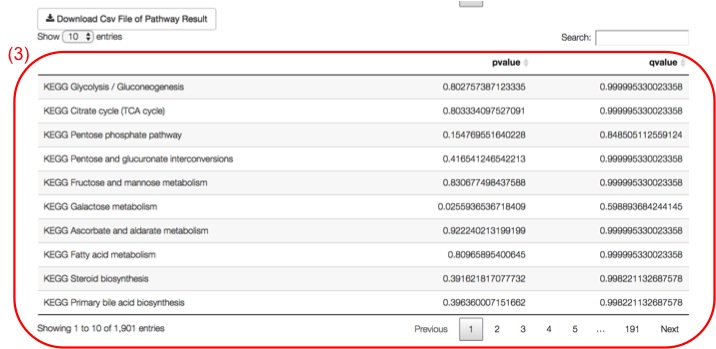
\includegraphics[scale=0.45]{./figure/metaDE/metaDEresult2.jpg}
\caption{``MetaDE" Results (2)}
\label{fig:MetaDEresult2}
\end{center}
\end{figure}

For the second step ``pathway analysis", there is (3) a tabular summary outputted, as shown in Figure \ref{fig:MetaDEresult2}. The summary includes the pathway names, the corresponding enrichment p-value and FDR. 
In addition to the results shown in the Browser, users can download the two tabular results to the working directory by clicking on "Download Csv File" on the top left of the summary table. 

